\chapter{Arhitektura i dizajn sustava}
		
		\textbf{\textit{dio 1. revizije}}\\

		Arhitektura programske potpore predstavlja strukturu sustava ili više njih koje sadrži elemente, njihova obilježja i odnose među njima. Temeljni razlozi definiranja arhitekture:		

	\begin{itemize}
		\item 	{poboljšava razumljivost i komunikaciju sudionika}
		\item 	{pomaže u donošenju temeljnih odluka pri izradi projekta}
		\item 	{omogućava rano uočavanje pogrešaka u oblikovanju}		
		\item         {moguće ponovno korištenje rješenja (engl. reuse)}
	\end{itemize}

	U konačnici, efikasno strukturiranje arhitekture programske potpore dovest će do poboljšanja kvalitete finalnog produkta projekta.

	\vspace{10mm} %10mm vertical space

	Arhitekturu našeg projekta možemo klasificirati na četiri ključna dijela koji osiguravaju izvršavanje naredbi korisnika: 
		
	\begin{packed_enum}
		\item 	{Web preglednik}
		\item 	{Web poslužitelj}
		\item 	{Web aplikacija}
		\item 	{Baza podataka}
	\end{packed_enum}			

		\begin{figure}[H]
					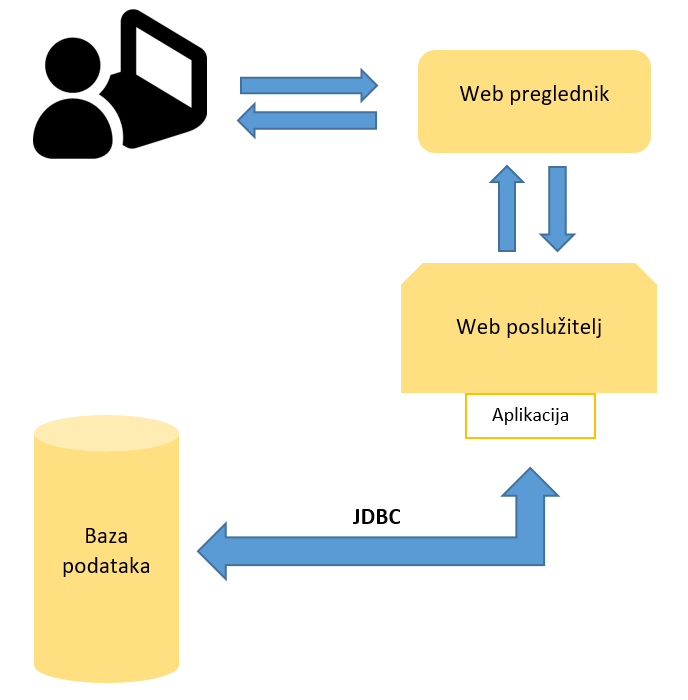
\includegraphics[scale=0.8]{arhitektura/arhitektura_sustava.png} %veličina slike u odnosu na originalnu datoteku i pozicija slike
					\centering
					\caption{Arhitektura sustava}
					\label{fig:arhitektura}
		\end{figure}

	\vspace{5mm} %5mm vertical space

		Najčešći model koji se koristi kod aplikacija je model klijent-poslužitelj pa tako koristimo i mi u našem projektu. Korisnik šalje upite, a poslužitelj odgovara na upite, dok i jedna i druga strana mogu imati korisničku i poslužiteljsku aplikaciju.

		\section{Baza podataka}
			
			\textbf{\textit{dio 1. revizije}}\\
			
		\textit{Potrebno je opisati koju vrstu i implementaciju baze podataka ste odabrali, glavne komponente od kojih se sastoji i slično.}
		
			\subsection{Opis tablica}
			

				\textit{Svaku tablicu je potrebno opisati po zadanom predlošku. Lijevo se nalazi točno ime varijable u bazi podataka, u sredini se nalazi tip podataka, a desno se nalazi opis varijable. Svjetlozelenom bojom označite primarni ključ. Svjetlo plavom označite strani ključ}
				
				\begin{longtabu} to \textwidth {|X[6, l]|X[6, l]|X[20, l]|}
					
					\hline \multicolumn{3}{|c|}{\textbf{korisnik - ime tablice}}	 \\[3pt] \hline
					\endfirsthead
					
					\hline \multicolumn{3}{|c|}{\textbf{korisnik - ime tablice}}	 \\[3pt] \hline
					\endhead
					
					\hline 
					\endlastfoot
					
					\cellcolor{LightGreen}IDKorisnik & INT	&  	Lorem ipsum dolor sit amet, consectetur adipiscing elit, sed do eiusmod tempor incididunt ut labore et dolore magna aliqua. Ut enim ad minim veniam 	\\ \hline
					korisnickoIme	& VARCHAR &   	\\ \hline 
					email & VARCHAR &   \\ \hline 
					ime & VARCHAR	&  		\\ \hline 
					\cellcolor{LightBlue} primjer	& VARCHAR &   	\\ \hline 
					
					
				\end{longtabu}
			
			
			\subsection{Dijagram baze podataka}
				\textit{ U ovom potpoglavlju potrebno je umetnuti dijagram baze podataka. Primarni i strani ključevi moraju biti označeni, a tablice povezane. Bazu podataka je potrebno normalizirati. Podsjetite se kolegija "Baze podataka".}
			
			\eject
			
			
		\section{Dijagram razreda}
		
			\textit{Potrebno je priložiti dijagram razreda s pripadajućim opisom. Zbog preglednosti je moguće dijagram razlomiti na više njih, ali moraju biti grupirani prema sličnim razinama apstrakcije i srodnim funkcionalnostima.}\\
			
			\textbf{\textit{dio 1. revizije}}\\
			
			\textit{Prilikom prve predaje projekta, potrebno je priložiti potpuno razrađen dijagram razreda vezan uz \textbf{generičku funkcionalnost} sustava. Ostale funkcionalnosti trebaju biti idejno razrađene u dijagramu sa sljedećim komponentama: nazivi razreda, nazivi metoda i vrste pristupa metodama (npr. javni, zaštićeni), nazivi atributa razreda, veze i odnosi između razreda.}\\
			
			\textbf{\textit{dio 2. revizije}}\\			
			
			\textit{Prilikom druge predaje projekta dijagram razreda i opisi moraju odgovarati stvarnom stanju implementacije}
			
			
			
			\eject
		
		\section{Dijagram stanja}
			
			
			\textbf{\textit{dio 2. revizije}}\\
			
			\textit{Potrebno je priložiti dijagram stanja i opisati ga. Dovoljan je jedan dijagram stanja koji prikazuje \textbf{značajan dio funkcionalnosti} sustava. Na primjer, stanja korisničkog sučelja i tijek korištenja neke ključne funkcionalnosti jesu značajan dio sustava, a registracija i prijava nisu. }
			
			
			\eject 
		
		\section{Dijagram aktivnosti}
			
			\textbf{\textit{dio 2. revizije}}\\
			
			 \textit{Potrebno je priložiti dijagram aktivnosti s pripadajućim opisom. Dijagram aktivnosti treba prikazivati značajan dio sustava.}
			
			\eject
		\section{Dijagram komponenti}
		
			\textbf{\textit{dio 2. revizije}}\\
		
			 \textit{Potrebno je priložiti dijagram komponenti s pripadajućim opisom. Dijagram komponenti treba prikazivati strukturu cijele aplikacije.}